%{- block documentheader %}
%{- if fontsize %}
\documentclass[%{{-fontsize-%}}]{article}
%{- else %}
\documentclass[12pt]{article}
%{- endif %}

% colors
\usepackage[usenames,dvipsnames]{xcolor}

% FONT setup
\usepackage{lmodern}
\renewcommand\familydefault{\sfdefault}
\usepackage[utf8]{inputenc}
\usepackage[T1]{fontenc}

\usepackage{tikz}
\usetikzlibrary{positioning}
% set styling for tikz nodes used throughout document
\tikzset{% 
    default picture/.style={%
        font=\normalsize, node distance=0em, outer sep=0em, inner sep=0em
    },
    default line/.style={%
        black!100, solid, thick
    },
    full width text/.style={%
        minimum height=1em, minimum width=7.2in, text width=7.2in, align=left
    }
}

\newcommand{\sandwich}{
  \tikz[]{
    \draw [gray, line width=1.5] (0ex,0.0ex) -- (2ex,0ex);
    \draw [gray, line width=1.5]  (0ex,0.75ex) -- (2ex,0.75ex);
    \draw [gray, line width=1.5] (0ex,1.5ex) -- (2ex,1.5ex);
}}

\newcommand{\thickdash}{
  \tikz[baseline=-0.75ex]{
    \draw [black, line width=0.75]  (0ex,0ex) -- (2ex,0ex);
}}

\newcommand{\thickcircle}{
  \tikz[baseline=-0.75ex]{
	  \draw [black, line width=0.5] (0ex,0ex) circle [radius=0.3ex];
}}

\usepackage{enumitem}
% set style for lists
\setlist[itemize]{itemsep=0pt, partopsep=0pt, topsep=0pt, label=\thickcircle, leftmargin=*}

\usepackage{calc}
\usepackage[paper=letterpaper, includefoot,
            top=0.5in, bottom=0.5in, 
            left=0.65in, right=0.65in]{geometry}

\setlength{\parindent}{0in}

% header, footer setup
\usepackage{fancyhdr,lastpage}
\pagestyle{fancy} 
\fancyhead{}
\fancyfoot{}
\fancyfoot{}
\renewcommand{\headrulewidth}{0pt}
\renewcommand{\footrulewidth}{0pt}

% PDF
\usepackage{hyperref}
\hypersetup{
pdfstartview={FitH},
pdftitle={Resume -- %{{contact.name | escape_tex  %}} },
pdfauthor=}},
pdfsubject={Resume for %{{ contact.name | escape_tex  %}}},
pdfcreator={pdflatex, resumepy},
pdfproducer={pdflatex, resumepy},
colorlinks=true,
linkcolor=Black,
urlcolor=Black
%linkcolor=Mahogany,
%urlcolor=Mahogany
}
%{- endblock documentheader %}

\begin{document}

%{ block contact -%}

\textbf{ %{{- contact.name | escape_tex -%}} }
\hfill \textbf{web:} \href{http://%{{- contact.web | escape_tex -%}} }{ %{{- contact.web | escape_tex -%}} }

\vskip-0.75em
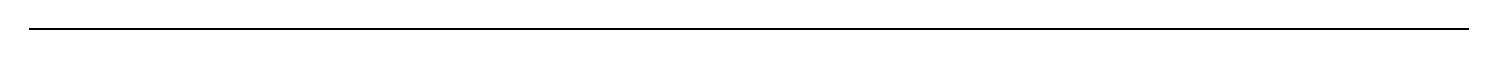
\begin{tikzpicture}[default picture]
\draw[default line] (0in, 0) -- (7.2in, 0);
\end{tikzpicture}

%{{contact.address | escape_tex -%}}, %{{ contact.city %}}, %{{contact.state %}} %{{ contact.zip %}} \\
\textbf{tel:} %{{ contact.phone %}} \textbf{email:} \href{mailto:%{{- contact.email -%}} }{ %{{- contact.email -%}} }
%{- endblock contact %}

%{ block education %}
\vskip1em
\sandwich~\textbf{Education}

%{ for school in education %}
\vskip0.5em
\textbf{ %{{- school.degree | escape_tex %}}, %{{ school.focus | escape_tex %}} } \hfill %{{ school.graduation %}} \\
\href{ %{{-school.web-%}} }{ %{{- school.schoolname | escape_tex -%}} }

%{- if school.notes %}
\vskip0.25em
\begin{itemize}
%{- for note in school.notes %}
  \item %{{ note | escape_tex | wordwrap %}} 
%{- endfor %}
\end{itemize}
%{- endif %}
%{ endfor %}
%{- endblock education %}


%{ block additional_education %}
%{- if additional_education %}
\vskip1em
\sandwich~\textbf{Additional Coursework}

%{ for school in additional_education %}
\vskip0.5em
\textbf{ %{{- school.course | escape_tex %}} } \hfill %{{ school.completed %}} \\
%{{school.schoolname%}}

%{- if school.notes %}
\vskip0.25em
\begin{itemize}
%{- for note in school.notes %}
  \item  %{{ note | escape_tex | wordwrap %}} 
%{- endfor %}
\end{itemize}
%{- endif %}
%{ endfor %}
%{- endif %}
%{- endblock additional_education %}


%{ block  work %}
\vskip1em
\sandwich~\textbf{Work Experience}

%{ for job in work %}
\vskip0.5em
\textbf{ %{{- job.position | escape_tex %}} } \hfill %{{ job.start %}} -- %{{ job.stop %}} \\
\href{ %{{- job.web -%}} }{ %{{- job.organization | escape_tex -%}} }

%{- if job.notes %}
\vskip0.25em
\begin{itemize}
%{- for note in job.notes %}
  \item %{{ note | escape_tex | wordwrap %}}
%{- endfor %}
\end{itemize}
%{- endif %}
%{ endfor %}
%{- endblock work %}


%{ block projects %}
%{- if projects %}
\vskip1em
\sandwich~\textbf{Projects}

%{ for project in projects %}
\vskip0.25em
\textbf{ %{{- project.title | escape_tex %}} } \hfill %{{ project.date %}} \\
\href{ %{{- project.web -%}} }{ %{{- project.web | escape_tex -%}} }
\vskip0.25em
%{- if project.notes %}
\begin{itemize}
%{- for note in project.notes %}
  \item  %{{ note | escape_tex | wordwrap  %}} 
%{- endfor %}
\end{itemize}
%{- endif %}
%{ endfor %}
%{- endif %}
%{- endblock projects %}


%{ block skills %}
\vskip1em
\sandwich~\textbf{Core Skills}

%{ for skill in skills %}
\vskip0.25em
\textbf{ %{{- skill.name | escape_tex %}} }
\vskip0.25em
\begin{itemize}
%{- for note in skill.notes %}
  \item %{{ note | escape_tex | wordwrap %}}
%{- endfor %}
\end{itemize}
%{ endfor %}

%{ endblock skills %}

\end{document}
